%!TEX root = ../main.tex
%%%%%%%%%%%%%%%%%%%%%%%%%%%%%%%%%%
% Links:
%
% Difficulty: Companies: 
%%%%%%%%%%%%%%%%%%%%%%%%%%%%%%%%%%

\chapter{Counts the items in the containers}
\label{ch:items_in_containers_amazon}
\section*{Introduction}
Imagine you are the owner of a successful online store. You would like to be able to query what is
the number of items you still have in the warehouse. The problem is that you cannot just walk into
the warehouse and count the items as they are stored in closed containers. Thankfully, the warehouse
is equipped with sensors and it is able to produce a string representing the state of the warehouse
and single containers. The problem described in this chapter investigates how we can write an
algorithm that takes such a string (the state of all the containers in the warehouse) and is able to
answer queries on the number of elements that are present in some portions of the warehouse itself. 

This problem has been reported to be asked during Amazon interviews and it is considered a medium
difficulty problem. We will investigate two solutions:
\begin{itemize}
	\item brute-force, that is going to have a relatively straightforward logic (blindly count the
	 items in the string) and be easy to code (in Section
	 \ref{items_in_containers_amazon:sec:bruteforce}),
	\item a more sophisticated one with optimal asymptotic complexity where the input string is
	preprocessed so that queries can be answered faster.
\end{itemize}



\section{Problem statement}
\begin{exercise}
	You are given a string $s$ representing the current state of a warehouse. The string contains
	only two kinds of characters: 
	\begin{description}
		\item[\bsq{\textbf{\texttt{*}}}(ASCII 42)]: representing an item 
		\item[\bsq{\textbf{\texttt{|}}}(ASCII 124)]: representing the boundaries of a container.
	\end{description}
	
	A container is a closed space within the warehouse and it is represented in $s$ by a pair of
	\bsq{\texttt{|}}. Items within a container $c$ are represented as \bsq{\texttt{*}} appearing
	withing the two \bsq{\texttt{|}} defining $c$. You are also given an array of pairs $Q = \{(s_0,
	e_0),(s_1, e_2),\ldots,(s_{n-1}, e_{e-1}) : 0 \leq s_i \leq e_i \leq |s|\}$, where each pair in
	$Q$ identifies a substring in $s$. Each element of $Q$ is a query you must answer to.
	
	Your task is to write a function that returns an array $A$ of length $n$, containing the answers
	to all of the queries in $Q$, where each element $A_i$ is the number of items contained in all
	the \textbf{closed} compartments between $(s_i, e_i)$.	

\begin{example}
	\hfill \\
	Given \texttt{s = \bsq{|**|*|*}} and $Q = \{(0,4),(0,5)\}$ the function returns $A=\{2,3\}$. $s$
	has a total of $2$ closed containers the first with $2$ and $1$ item inside respectively.
	
	The first query asks you to find the number of elements in the substring $s[0,4]=$
	\texttt{\bsq{|**|*}} where three items are represented but only two are within a closed
	container (the first two).
	
	The second query refers to the substring $s[0,5]=$ \texttt{\bsq{|**|*|}}. The items are the same
	as in the previous query but this time all of them are in closed containers.
	
\end{example}

\begin{example}
	\hfill \\
	Given \texttt{s = \bsq{*|*|}} and $Q = \{(0,2),(1,3)\}$ the function returns $A=\{0,1\}$. $s$
	has a total of two items and only $1$ closed container containing only a single item.

	The first query refers to the substring $s[0,2]=$ \texttt{\bsq{*|*}}. No closed container are
	represented in such substring thus the answer in this case must be $0$. However, the second
	question refers to  $s[1,3]=$ \texttt{\bsq{|*|}} where we can see we have a valid container. We
	can therefore counts the elements in it.
\end{example}

\end{exercise}
\section{Clarification Questions}

\begin{QandA}
	\item Is it guaranteed for the input string $s$ to only contains valid character?
	\begin{answered}
		\textit{Yes, you do not need to worry about the sanity of the input.}
	\end{answered}
\end{QandA}

\section{Discussion}
\label{items_in_containers_amazon:sec:discussion}



\subsection{Brute-force}
\label{items_in_containers_amazon:sec:bruteforce}
This problem has a straightforward solution that basically loops over all the elements  specified in
a query $(s,e) \in Q$ and counts all the elements inside the containers. Because the $|s-e|$ is
$O(|s|)$ the complexity of this approach is $O(|s|*|Q|)$. Listing
\ref{list:items_in_containers_amazon_bruteforce} shows an implementation of such idea. Notice that
most of the code complexity of this solution is in the \inline{count_items_in_substring} function
that has to make sure only to count items that are within a closed container. It does so by first
finding the first container wall appearing after the start of the query interval. We can safely skip
all those items because there are not inside a container. Once we have found the beginning of the
first container, we can proceed by counting the elements, one container   at the time. 
\lstinputlisting[language=c++, caption={Na\"ive solution to the \textit{items in the container} problem.},label=list:items_in_containers_amazon_bruteforce]{sources/items_in_containers_amazon/items_in_containers_amazon_solution1.cpp}

\subsection{Linear time solution}
\label{items_in_containers_amazon:sec:lineartime}
There is however a much faster solution to this problem that can be easily implemented provided we
have come precomputed values. Performing some pre-computation in order to speed-up an algorithm is a
common idea that is useful for the solution of many coding interview questions. In this particular
problem, we are going to calculate two values for each character of the input string:
\begin{description}
	\item[$C_i$, \textbf{the closest delimiter to the right}]: we want to have for each character $s_i$ of
	the input string $s$ the information about the index of the closest container delimiter
	appearing after it. In other words we are looking for the index $j > i$ such that $s[j]='|'$. If
	such index does not exists then we assume it is the index of the last character of $s$, i.e.
	$|s|-1$.
	\item[$P_i$,  \textbf{the number of elements in all containers to the left}]: this value should answer
	the question: given a character at index $i$ of $s$, how many items are placed into all the
	closed containers appearing to the left of $i$? 
\end{description}
When this information is available for each and every position of $s$ then we can answer each query in constant time.
Given a query $(l,r)$, we can calculate the answer to it by using the information about 
the closest container delimiter to the right of $l$, $c\geq l$,
to find the beginning of the first container in the range $(s,e)$. All the elements 
between $l$ and $c$ can be ignored.
So now that we have basically transformed our query from $(l,r)$ to $(c,r)$ we are ready to use the prefix sum of the number of elements 
in the containers.

We can calculate the answer to $(c,r)$ by simply returning  $P_r - P_l$: the number of elements in the all container up to index $r$ minus, 
the number of elements in all containers up to the index $l$. 


Figure \ref{fig:items_in_containers_amazon:example_prefix} shows the values of $P$ and $C$ for the input string is \inline{s="|**|*|*"}.
Each value of the array $P_i$ contains the count of the items inside all the containers in the prefix of $s$ u to and including index $i$. 
For instance $P_4=2$ because the substring of $s$ between indices $0$ and $4$ only contains one container with two elements in it while $P_5=3$ because
between indices $0$ and $5$we have two containers with $2$ and $1$ items inside, respectively.
The values in $C_i$ contains the indices of the first character \inline{'|'} in the suffix of $s$ from index $i$.
For instance $C_1=3$ because the first \inline{'|'} after index $1$ appears at index $3$ in $s$ while
$C_3=3$ because $s[3]$ contains \inline{'|'} itself.
Notice that the last element of $s$ always contains $|s|-1$ regarless of the fact $s_{|s|-1}$ is \inline{'|'} or not. 
Listing \ref{list:items_in_containers_amazon_lineartime} shows an implementation of the idea above. 
The main driver function is \inline{items_in_containers_lineartime} which first calls other two functions:
\begin{enumerate*}
	\item \inline{find_closest_bars_right} and,
	\item \inline{prefix_sum_containers_items}
\end{enumerate*}
that are responsible for the pre-computation of $C$ and $P$, respectively.
Notice that in Listing \ref{list:items_in_containers_amazon_lineartime}, 
for the sake of clarity, $C$ and $P$, are named \inline{closest_bars_right} and \inline{prefix_sum_count_items}, respectively.

\begin{figure}
	\centering
	\begin{subfigure}[t]{0.48\textwidth}
		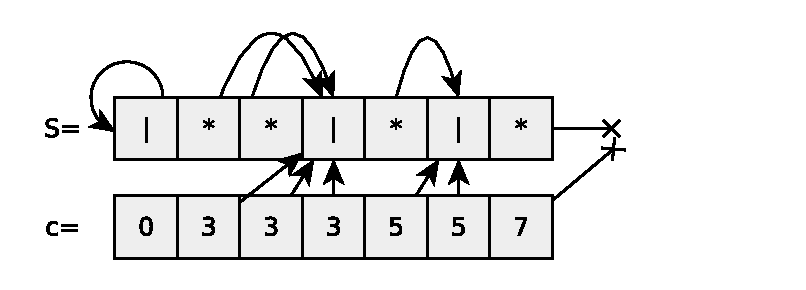
\includegraphics[width=1\linewidth]{sources/items_in_containers_amazon/images/delimiter_on_right}
		\caption{Each element at location $i$ of the array $C$ contains an integer corresponding to the smallest index $j$ of $s$ larger than $i$ such that $s[j]='|'$ is a delimiter of a container.}
		\label{fig:items_in_containers_amazon:delimiter_right}
	 \end{subfigure}
	\hfill
	\begin{subfigure}[t]{0.48\textwidth}
		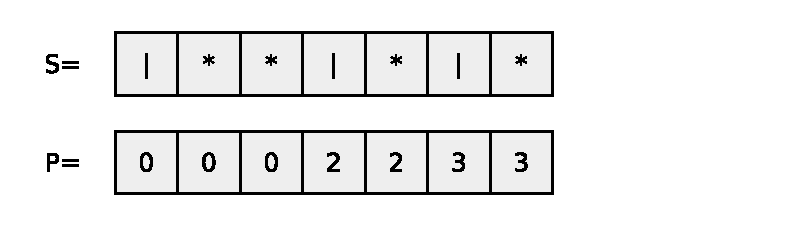
\includegraphics[width=1\linewidth]{sources/items_in_containers_amazon/images/prefix_sum}
		\caption{Each element at index $i$ of the array $P$ contains the number of elements in all the closed containers appearing before $i$ in $s$.  }
		\label{fig:items_in_containers_amazon:prefix_sum}
	 \end{subfigure}
	 \label{fig:items_in_containers_amazon:example_prefix}
\end{figure}	 


\lstinputlisting[language=c++, caption={Linear time and linear space solution to the \textit{items in the container} problem.},label=list:items_in_containers_amazon_lineartime]{sources/items_in_containers_amazon/items_in_containers_amazon_solution2.cpp}